%%%%%%%%%%%%%%%%%%%%%%%% ExtendedAbstract.tex %%%%%%%%%%%%%%%%%%%%%%%%
%                                                                    %
%  Template for the 10-page extended abstract to be submitted for    %
%  the MSc degree conferral at Instituto Superior Tecnico.           %
%                                                                    %
%  Author:                                                           %
%                                                                    %
%       Andre C. Marta                                               %
%       Area Cientifica de Mecanica Aplicada e Aeroespacial          %
%       Departamento de Engenharia Mecanica                          %
%       Instituto Superior Tecnico                                   %
%       Av. Rovisco Pais                                             %
%       1049-001 Lisboa                                              %
%       Portugal                                                     %
%       Tel: +351 21 841 9466                                        %
%                        3466 (extension)                            %
%       Email: andre.marta@ist.utl.pt                                %
%                                                                    %
%  Created:       Dec  2, 2011                                       %
%  Last Modified: Dec 27, 2011                                       %
%%%%%%%%%%%%%%%%%%%%%%%%%%%%%%%%%%%%%%%%%%%%%%%%%%%%%%%%%%%%%%%%%%%%%%
% This document uses the LaTeX class file "article.cls"              %
%%%%%%%%%%%%%%%%%%%%%%%%%%%%%%%%%%%%%%%%%%%%%%%%%%%%%%%%%%%%%%%%%%%%%%
\documentclass[8pt,a4paper,twocolumn]{article}

%%%%%%%%%%%%%%%%%%%%%%%%%%%%%%%%%%%%%%%%%%%%%%%%%%%%%%%%%%%%%%%%%%%%%%
% Document preamble
%%%%%%%%%%%%%%%%%%%%%%%%%%%%%%%%%%%%%%%%%%%%%%%%%%%%%%%%%%%%%%%%%%%%%%

%% Builds upon the graphics  package, providing a key-value interface
%% for optional arguments to the \includegraphics command that go far
%% beyone what the graphics package offers.
%% http://www.ctan.org/tex-archive/help/Catalogue/entries/graphicx.html
%% if you use PostScript figures in your article
%% use the graphics package for simple commands
%% \usepackage{graphics}
%% or use the graphicx package for more complicated commands
%% \usepackage{graphicx}
%% or use the epsfig package if you prefer to use the old commands
%% \usepackage{epsfig}
\usepackage{graphicx} % Enhanced LaTeX Graphics
\usepackage{siunitx}

%Tipo de letra Arial
\usepackage{helvet}
\renewcommand{\familydefault}{\sfdefault}

% acentos e cedilhas
\usepackage[utf8]{inputenc}
%\usepackage[T1]{fontenc}

% Multiple figures
%\usepackage{subfigure} % subcaptions for subfigures
%\usepackage{subfigmat} % matrices of similar subfigures

\usepackage[font=footnotesize, skip = 1pt, labelfont=bf]{caption}
\usepackage[font=footnotesize]{subcaption}

% Declaring new column types
% 'dcolumn' package defines D to be a column specifier with
% three arguments: D{<sep.tex>}{<sep.dvi>}{<decimal places>}
%                  D{<sep.tex>}{<sep.dvi>}{<left digit places>.<right digit places>}
\usepackage{dcolumn}           % decimal-aligned tabular math columns
% d takes a single argument specifying the number of decimal places, e.g., d{2}
% or the number of digits to the left and right of the seperator, e.g., d{3.2}
\newcolumntype{.}   {D{.}{.}{-1}} % column alignedd on the point separator '.'
\newcolumntype{d}[1]{D{.}{.}{#1}} % column centered on the point separator '.'
\newcolumntype{e}   {D{E}{E}{-1}} % column centered on the exponent 'E'
\newcolumntype{E}[1]{D{E}{E}{#1}} % column centered on the exponent 'E'

%% American Mathematical Society (AMS) plain Tex macros
%%
%% The amsmath package is the principal package in the AMS-LaTeX distribution
%% http://www.ctan.org/tex-archive/help/Catalogue/entries/amsmath.html
\usepackage{amsmath}
\DeclareMathSizes{7}{7}{3}{3} 
\usepackage{pifont}
%%
%% The amsfonts package provides extended TeX fonts
%% http://www.ctan.org/tex-archive/help/Catalogue/entries/amsfonts.html
\usepackage{amsfonts}
%% The amssymb package provides various useful mathematical symbols
\usepackage{amssymb}
%%
%% The amsthm package provides extended theorem environments
%% http://www.ctan.org/tex-archive/help/Catalogue/entries/amsthm.html
\usepackage{amsthm}

%% Improves the interface for defining floating objects such as figures and tables.
%% The package also provides the H float modifier option of the obsolete here package.
%% http://www.ctan.org/tex-archive/help/Catalogue/entries/float.html
\usepackage{float}

%% Control sectional headers. 
%% http://www.ctan.org/tex-archive/help/Catalogue/entries/sectsty.html
\usepackage{sectsty}
%%
%% Redefine the font size of the 'section' and 'subsection' headings
\newcommand{\myFontSize}{\fontsize{9}{0}\selectfont}
\sectionfont{\myFontSize}       % 10pt, Bold face (default)
\subsectionfont{\myFontSize} % 10pt, Plain face

%% Select alternative section titles.
%% http://www.ctan.org/tex-archive/help/Catalogue/entries/titlesec.html
\usepackage{titlesec}
\usepackage{booktabs}
%\usepackage{multirow}
%\usepackage{array}
\usepackage{csquotes}% Recommended
%\usepackage[style=authoryear, backend=bibtex, doi=false,isbn=false,url=false,eprint=false,dashed=false,maxcitenames=2, maxbibnames=100]{biblatex}
%\addbibresource{library.bib}

%%
%% Left indent, before and after spacing
%% (The starred version kills the indentation of the paragraph following the title)
\titlespacing*{\section}{0pt}{10pt}{0pt}
\titlespacing*{\subsection}{0pt}{10pt}{0pt}

%% Section numbers with trailing dots. 
%% http://www.ctan.org/tex-archive/help/Catalogue/entries/secdot.html
\usepackage{secdot}
\usepackage{epstopdf}
%%
%% Also put a dot after the subsection number
\sectiondot{subsection}
%% Set a space between dot and heading text
\sectionpunct{section}{. }    % By default, \sectiondot places a \quad
\sectionpunct{subsection}{. } % after the number

% These are exact settings for a A4 page with top margin of
% 25 mm, bottom margin of 30 mm, left and right margins of 25 mm,
% printable area 242 X 160 mm.

\setlength{\topmargin}{-10.4mm}
\setlength{\headheight}{0.0mm}
\setlength{\headsep}{10.0mm}
\setlength{\textwidth}{160mm}
\setlength{\textheight}{242mm}
\setlength{\oddsidemargin}{0mm}
\setlength{\evensidemargin}{0mm}
\setlength{\marginparwidth}{0mm}
\setlength{\marginparsep}{0mm}

% New command to refer to equations as Eq.(1),Eq.(2),...
\newcommand{\eqnref}[1]{Eq.(\ref{#1})}

%%%%%%%%%%%%%%%%%%%%%%%%%%%%%%%%%%%%%%%%%%%%%%%%%%%%%%%%%%%%%%%%%%%%%%%%%%%%%%%%%%%%%%%%
% Title, authors and addresses

\title{\bfseries Optimization in Architecture}
\date{May 2019}
\author{Catarina Belém\\ catarina.belem@tecnico.ulisboa.pt \\ \\ Instituto Superior Técnico, Lisboa, Portugal}

%%%%%%%%%%%%%%%%%%%%%%%%%%%%%%%%%%%%%%%%%%%%%%%%%%%%%%%%%%%%%%%%%%%%%%%%%%%%%%%%%%%%%%%%
\begin{document}

% Begin one column section for title and abstract
%
% http://www.faqs.org/faqs/de-tex-faq/part5/
\twocolumn[
\begin{@twocolumnfalse}
\maketitle

	%%%%%%%%%%%%%%%%%%%%%%%%%%%%%%%%%%%%%%%%%%%%%%%%%%%%%%%%%%%%%%%%%%%%%%
%     File: ExtendedAbstract_abstr.tex                               %
%     Tex Master: ExtendedAbstract.tex                               %
%                                                                    %
%     Author: Andre Calado Marta                                     %
%     Last modified : 2 Dez 2011                                     %
%%%%%%%%%%%%%%%%%%%%%%%%%%%%%%%%%%%%%%%%%%%%%%%%%%%%%%%%%%%%%%%%%%%%%%
% The abstract of should have less than 500 words.
% The keywords should be typed here (three to five keywords).
%%%%%%%%%%%%%%%%%%%%%%%%%%%%%%%%%%%%%%%%%%%%%%%%%%%%%%%%%%%%%%%%%%%%%%

%%
%% Abstract
%%
\begin{abstract}

Sed ut perspiciatis unde omnis iste natus error sit voluptatem accusantium doloremque laudantium, totam rem aperiam, eaque ipsa quae ab illo inventore veritatis et quasi architecto beatae vitae dicta sunt explicabo. Nemo enim ipsam voluptatem quia voluptas sit aspernatur aut odit aut fugit, sed quia consequuntur magni dolores eos qui ratione voluptatem sequi nesciunt. Neque porro quisquam est, qui dolorem ipsum quia dolor sit amet, consectetur, adipisci velit, sed quia non numquam eius modi tempora incidunt ut labore et dolore magnam aliquam quaerat voluptatem. Ut enim ad minima veniam, quis nostrum exercitationem ullam corporis suscipit laboriosam, nisi ut aliquid ex ea commodi consequatur? Quis autem vel eum iure reprehenderit qui in ea voluptate velit esse quam nihil molestiae consequatur, vel illum qui dolorem eum fugiat quo voluptas nulla pariatur?

Sed ut perspiciatis unde omnis iste natus error sit voluptatem accusantium doloremque laudantium, totam rem aperiam, eaque ipsa quae ab illo inventore veritatis et quasi architecto beatae vitae dicta sunt explicabo. Nemo enim ipsam voluptatem quia voluptas sit aspernatur aut odit aut fugit, sed quia consequuntur magni dolores eos qui ratione voluptatem sequi nesciunt. Neque porro quisquam est, qui dolorem ipsum quia dolor sit amet, consectetur, adipisci velit, sed quia non numquam eius modi tempora incidunt ut labore et dolore magnam aliquam quaerat voluptatem. Ut enim ad minima veniam, quis nostrum exercitationem ullam corporis suscipit laboriosam, nisi ut aliquid ex ea commodi consequatur? Quis autem vel eum iure reprehenderit qui in ea voluptate velit esse quam nihil molestiae consequatur, vel illum qui dolorem eum fugiat quo voluptas nulla pariatur?
\\
%%
%% Keywords (max 5)
%%
\noindent{{\bf Keywords:}} Demo word, Lorem, Ipsum \\

\end{abstract}



\end{@twocolumnfalse}
]
	\section{Introduction}
\label{sec:intro}

Lorem ipsum dolor sit amet, consectetur adipiscing elit, sed do eiusmod tempor incididunt ut labore et dolore magna aliqua. Ut enim ad minim veniam, quis nostrud exercitation ullamco laboris nisi ut aliquip ex ea commodo consequat. Duis aute irure dolor in reprehenderit in voluptate velit esse cillum dolore eu fugiat nulla pariatur. Excepteur sint occaecat cupidatat non proident, sunt in culpa qui officia deserunt mollit anim id est laborum.

Lorem ipsum dolor sit amet, consectetur adipiscing elit, sed do eiusmod tempor incididunt ut labore et dolore magna aliqua. Ut enim ad minim veniam, quis nostrud exercitation ullamco laboris nisi ut aliquip ex ea commodo consequat. Duis aute irure dolor in reprehenderit in voluptate velit esse cillum dolore eu fugiat nulla pariatur. Excepteur sint occaecat cupidatat non proident, sunt in culpa qui officia deserunt mollit anim id est laborum.\cite{Spalding1972}

	% A Theory section should extend, not repeat, the background to the
% article already dealt with in the Introduction and lay the foundation for further work.
\section{Optimization}
\label{sec:backg}
An optimization process consists in two main parts: the model of the problem to be optimized and the optimization algorithm. The creation of the model involves the definition of variables, objective functions, and, optionally, constraints. In architectural design optimization, the variables are the parameters whose value will be modified, objective functions represent the performance criteria that we aim to optimize, and constraints are the conditions on the parameters that must be satisfied so that a solution is valid for the defined problem.

Depending on the number of objectives, optimization problems can be classified as \ac{SOO} or \ac{MOO}. The former focuses on the optimization of one objective, whilst the latter focuses on more complex problems that involve multiple objectives.
Despite the increased complexity, \ac{MOO} encloses benefits, such as the visualization of the trade-offs among the different objectives and the selection of the solution that better fits the users' needs. This can be achieved through Pareto-based optimization, an approach that finds the solutions for which it is impossible to improve an objective value without deteriorating others. These solutions are called nondominated and represent the Pareto front. 

% Typically building design involves multiple conflicting objectives, such as maximum lighting comfort \textit{versus} maximum thermal comfort, or minimum energy consumption \textit{versus} maximum thermal comfort. When confronted with the optimal solutions returned by Pareto-based optimization, architects can compare the different design options according to different performance criteria, and, thus, make more informed decisions about the different compromises involved. However, this approach presents some drawbacks towards its application, namely, the requirement for a larger number of function evaluations and the difficulties in the visual representation of optimal solutions when the number of objectives is greater than three.

\subsection{Optimization Algorithms}
Optimization algorithms can be classified differently according to their properties. Considering the extent of the search, algorithms can be distinguished into local or global. Local optimization algorithms strive to find a solution for which the objective function yields a better value than for all the other solutions in its vicinity, i.e., a local optimum. These algorithms are usually highly sensitive to the starting point of the search and they tend to focus on smaller regions of the solution space. Conversely, global optimization algorithms strive to find globally optimal solutions, i.e., the best of all the local optima. To this end, these algorithms explore larger regions of the solution space, requiring a larger number of evaluations. However, this can be problematic for problems involving expensive objective functions. In these cases, one can apply a global algorithm to identify a promising region and then a local algorithm to more rapidly converge towards the optima within that region. 

A second classification differentiates deterministic and stochastic algorithms. Given the same starting point and configuration, deterministic algorithms systematically apply the same sequence of steps and, as a consequence, they always return the same result. In contrast, stochastic algorithms include some form of randomness and, therefore, often yield different results for the same starting point and algorithm's configuration.

The final distinction is between derivative-based and derivative-free algorithms, depending on their use of information about the objective functions' derivatives (e.g., the direction and magnitude of its greatest increase). 

In \ac{BPO}, the objective function tends to be simulation-based and, thus, does not have an analytical form. In these cases, it is not possible to apply derivative-based optimization algorithms. While, ideally, one could apply finite-difference algorithms to approximate the derivatives, this would require several extra simulations, which becomes impractical for problems involving expensive objective functions. Instead, one must resort to derivative-free optimization algorithms, which treat the objective functions as \textit{black-boxes} \cite{Rios2013}.

The following subsections describe three classes of derivative-free algorithms according to the classification proposed in the context of architectural design \cite{Wortmann2017ADO}, which first subdivides the algorithms according to the search strategy's determinism, namely, metaheuristics and iterative algorithms, and then partitions the latter into direct-search and model-based algorithms, based on the function explored to guide the search. 

\subsection{Direct-search Algorithms}
Direct-search algorithms iteratively evaluate a sequence of candidate solutions, proposed by a deterministic strategy, and select the best solution obtained up to that moment \cite{Conn2009}. They are regarded as valuable tools to address complex optimization problems, not only because most of them were proved to rely on solid mathematical principles, but also due to their good performance at initial stages of the search process \cite{Rios2013}. 

The main limitations of these algorithms are their performance deterioration with an increasing number of input variables and their slow asymptotic convergence rates as they get closer to the optimal solution \cite{Kolda2003}. Despite the existence of algorithms and benchmarks comparing \ac{SOO} direct-search algorithms \cite{Wortmann2017GABESTCHOICE,Waibel2018}, only recently have these started to appear in the context of \ac{MOO}~\cite{Custodio2010}.

Undoubtedly, one of the most relevant direct-search algorithms is the \textit{\ac{NMS}} \cite{Nelder1964}, a local \ac{SOO} direct-search algorithm. The \textit{\ac{NMS}} algorithm envelopes a region of the design space using a simplex, which is a generalization of a triangle to arbitrary dimensions, which is then successively modified using geometric operations that replace the simplex's worst vertex values.

Another interesting simplex-based algorithm is \textit{SUBPLEX} \cite{Rowan1990}, which attempts to overcome the \textit{\ac{NMS}} difficulties when addressing higher dimensional problems by decomposing the problem in low\nobreakdash-\hspace{0pt}dimensional
subspaces. The most promising ones are then explored by \textit{\ac{NMS}}.

Differently from the previous local algorithms, \textit{\ac{DIRECT}} \cite{Jones1993DIRECT} is a global \ac{SOO} algorithm, which recursively subdivides the design space into smaller multidimensional hyper-rectangles, each represented by a solution in their center. For each solution, the objective function is evaluated, thus yielding an estimate of the quality of each rectangle. Based on these values, \textit{\ac{DIRECT}} focus the search on more promising regions of the design space, further subdividing those. \textit{\ac{DIRECT}-L} \cite{Gablonsky2001} is a modification of \textit{\ac{DIRECT}} that minimizes the overall number of function evaluations, making it more efficient for functions with few local optima and a single global optimum. 

\textit{\ac{DMS}} \cite{Custodio2010} is a global multi-objective direct-search algorithmic framework which combines the main ideas of directional direct-search algorithms with Pareto dominance concepts. In simple terms, \textit{\ac{DMS}} maintains a list of feasible nondominated solutions and their associated step sizes, from which it iteratively evaluates a few solutions along a predefined set of directions located at a distance determined by the solution's step size. The list is updated when better solutions are found. Otherwise, the step size is reduced. The process then repeats. 

Overall, direct-search algorithms are not as popular as other classes of derivative-free algorithms. Nevertheless, their convergence proofs and the recent developments in the field of \ac{MOO} make this class very appealing for \ac{BPO}. 

\subsection{Metaheuristics Algorithms}
Metaheuristics are algorithms that rely on randomization, and biological or physical analogies to locate good solutions in complex design spaces \cite{Glover2003Metaheuristics}. Their non-deterministic and inexact nature confer them the ability to handle complex and irregular objective functions.

Metaheuristics can be good optimization algorithms when provided with sufficient amounts of time to do the necessary objective function evaluations \cite{Conn2009}. Unfortunately, this is not possible in architecture, where each evaluation can be a time-consuming simulation. However, because of their stochastic nature, limiting the number of evaluations has repercussions on the convergence guarantees \cite{Hasancebi2009}.

Depending on the metaphors adopted by each algorithm, metaheuristics can be classified in different subclasses, including, \acp{EA}, which explore natural selection and evolution concepts (e.g., reproduction, recombination, crossover, and mutation), Swarm algorithms, which explore collective intelligence through the cooperation of homogeneous agents in the environment (e.g., birds), and Physical Algorithms, which take inspiration from physical processes (e.g., the annealing process in metallurgy) \cite{Glover2003Metaheuristics}.

% GA Explained
The \textit{\ac{GA}} is an \ac{EA} that explores biological evolution to search for better solutions. It randomly generates an initial set of individuals representing the candidate solutions, called population, which is then evolved for a specified number of iterations (or generations). The evolution process is comprised of four main phases: (1) adaptability, where individuals of the population are assigned a suitability or fitness value; (2) mating selection, where pairs of individuals are selected for reproduction based on a probabilistic function; (3) crossover, where the variables' values of the selected individuals are recombined to produce new individuals; and (4) mutation, where new individuals are subjected to random copying errors with a certain probability. While in earlier generations, populations are usually more diverse, in final generations, their individuals are often similar to the fittest individuals, thus emulating the natural selection mechanism \cite{Glover2003Metaheuristics}.

% NSGA-II
Along the same line, \textit{\ac{NSGA-II}} is a \textit{\ac{GA}} specially tailored for \ac{MOO} problems, which incorporates the ideas of population genetics and evolution, Pareto dominance, and a crowding measure to attain an approximation of the Pareto front that is both accurate and diverse \cite{Deb2002}. In simple terms, \textit{\ac{NSGA-II}} maintains an archive and a population, which are iteratively evolved until a stopping criteria is met. Every iteration, the algorithm combines the archive and the population and sorts their individuals according to their nondomination ranks, a measure of the number of Pareto fronts that have to be removed until an individual becomes nondominated. Individuals belonging to the same rank are also sorted according to a density measure, based on the average distance of their two closest individuals. Afterwards, the archive is replaced with the best $50\%$ individuals and the next offspring produced based on the recombination and mutation of the individuals in the archive.

% PSO
Although less explored, \ac{PSO} algorithms have also been shown promising results in some optimization problems, surpassing widely reputed \acp{EA}. In their simpler versions, \ac{PSO} algorithms are global algorithms inspired by biological systems, such as the collective behavior of flocking birds, which interact and learn from one another to solve problems. In \ac{PSO}, the intelligence is decentralized, self-organized, and distributed throughout the participating particles (or swarm), which maintain information about their velocity, current and individual best positions, and also the global best position known to the swarm. At each time step, the position and velocity of each particle are updated according to the position of the best swarm or close neighbor \cite{Glover2003Metaheuristics}.
	
Overall, metaheuristics are stochastic algorithms, mostly without convergence guarantees, usually requiring several hundreds or even thousands of evaluations in order to obtain good solutions. For problems involving expensive objective functions, like most architectural optimization problems, and especially for \ac{MOO} problems, these algorithms are usually not a good choice. Unfortunately, there is a predominance of these algorithms (e.g., \textit{\ac{GA}} and \textit{\ac{NSGA-II}}) among \ac{BPO} practitioners \cite{Wortmann2017GABESTCHOICE}, with very few optimization tools supporting other classes of algorithms. Nevertheless, they can be very efficient solvers when properly configured. However, the optimal set of parameters is problem-specific and the same configuration applied to another problem might yield a bad performance.

\subsection{Model-based Algorithms}
Model-based algorithms replace the original objective functions with approximations. These approximations, called the surrogates, are generated from a limited set of known objective function values and can then be efficiently explored to determine the promising candidate solutions to evaluate next. These evaluations are then used to improve the surrogates and this process is repeated until a stopping condition is satisfied \cite{Koziel2011}. 

% Nowadays, the techniques applicable to the generation of surrogate models range from trust-region methods to \ac{ML} techniques. These techniques can be used to create (1) local surrogates, i.e., models where the approximation to the objective function is built around a certain point, and (2) global surrogates, i.e, models where the approximation is generated from all the obtained points. Whilst the former relies on the construction of simple, partial models of the objective function, the latter relies on the creation of a full model, which requires balancing the need for improving the model's accuracy by exploring broader regions in the solution space with the need for improving the objective function's value by exploiting promising regions~\cite{Koziel2011}. This balance is determined by a strategy that selects the next promising solutions to evaluate. 

Undoubtedly, the best feature of model-based algorithms is the reduction in total optimization time. This is particularly relevant in the context of \ac{BPO}, which involves time-consuming objective functions. Notwithstanding the existence of different studies involving \ac{ML} techniques for the creation of surrogate models~\cite{Koziel2011}, including \ac{MLP} and \textit{\ac{RBF}}, only a few have actually been applied in the context of architecture. This scenario is even more self-evident when we shift from the single- to the multi-objective optimization context.

Two relevant local model-based algorithms are \textit{\ac{COBYLA}} and \ac{BOBYQA}. The former uses a simplex to iteratively generate linear approximations of the objective function, whereas the latter generates quadratic approximations instead \cite{Powell1994COBYLA, Powell2009BOBYQA}.

\ac{RBF}-based algorithms create a global approximation of the objective function as the weighted sum of radial basis functions, whose weights are estimated based on the interpolation of previous evaluation results and are iteratively updated to improve the approximation.

When compared with metaheuristics, global model-based algorithms exhibit very good performance at initial stages of an optimization process, allowing for considerable speedups in the overall optimization.
	\section{Algorithmic Optimization in Architecture}
\label{sec: Methodology}

With the ability to quickly update a design, to generate the corresponding analytical model, and, finally, to automatically evaluate the design in an analytical tool, it becomes possible to implement automated optimization processes. We name these processes \ac{AO}.

\ac{AO} treats the analyses' results for different variations of the design as the functions to optimize, i.e., as the objective functions. These functions have a domain which corresponds to the range of acceptable designs as specified by the architect. Moreover, since we do not know their mathematical form, these objective functions are often treated as black- boxes, and, as a result, information about the their derivatives cannot be extracted. For this reason, methods depending on function derivatives cannot be used to address this problem. Instead, we use derivative-free (or black-box) algorithms, which can be divided into three distinct subclasses: direct-search, metaheuristics, and model-based \cite{Conn2009,Glover2003Metaheuristics,Koziel2011}.

\todo{TRABALHAR NA TRANSIÇÃO}

	\section{Case Studies}
\label{sec:resul}
Given that the framework makes several optimization algorithms available, the effectiveness of the framework is highly dependent on the effectiveness of these algorithms. This section focus on the evaluation of these algorithms on a series of computationally complex optimization problems within the architectural practice. This paper presents and evaluates two of those problems, a single- and a multi-objective optimization of simulation-based lighting and structural aspects of buildings.

When measuring the optimization algorithms' performance, several factors must be considered: (1) the optimization time is sensitive to the computational power of the machine where the algorithm is being run, (2) the non-determinism of several algorithms, and (3) the algorithms' hyperparameters. Firstly, to remove the time dependency of the machine characteristics and objective function's complexity, we measure the performance of the optimization algorithm in terms of the number of function evaluations, which is proportional to the actual time spent by the optimization process. Secondly, the stochastic nature of several optimization algorithms (e.g., random initial points, random modifications to solutions) might yield different results even when ran twice under the same configurations. To address this limitation, we run each stochastic algorithm three times and we use the average of the values to draw conclusions. Finally, for each problem, the algorithm's performance can be better or worse depending on its configurations. To this end, we opt for using the default algorithm's configurations, thus emulating the case when the architect's knowledge does not suffice to properly fine-tune the algorithm. 

All tests were run on a dual \textit{Intel Xeon CPU E5-2670 @ 2.60GHz with 64GB RAM}, where each daylight and structural simulation take approximately $7$ minutes and $40$ seconds to complete, respectively.

\subsection{Single-Objective Optimization: Ericeira House}
The first case study involved the optimization of the daylight conditions of a room in an isolated private house in Portugal~\cite{Caetano2018}. The room was designed with a set of façade shading panels that modulate the daylight conditions on the interior of the room. The panels are composed of a set of horizontal wood bars of different sizes, which alternate between one full-length bar and a set of smaller bars. For aesthetics reasons, the size and position of the smaller bars along the panel's width were randomized. The final pattern of the façade's shading panels was defined in terms of the length’s step, the maximum distance separating two consecutive bars, and the minimum and maximum lengths of the smaller bars. Initially, the goal was to find a solution for the shading panels that maximized the room's daylight performance, which was measured using the \ac{sUDI} metric \cite{Nabil2006}. While, in general, it is known that the more openings in the shading panels, the more daylight enter the room, this may also cause situations of uncomfortable glare. As a result, these situations should be accounted for, and, notwithstanding the values of the optimization process, architects should always perceive optimization results with a critical thinking. \Cref{fig:ericeira_multiple_panels} represents some design variations, ranging from denser patterns, with lower \ac{sUDI} values, to sparser ones, with higher \ac{sUDI} values.

\begin{figure}[htpb]
	\centering
	\includegraphics[width=\columnwidth]{../report/Images/Evaluation/Ericeira_2.png}
	\caption[Ericeira Solarium: Different representations of the shading panels’ geometric pattern]{Ericeira Solarium: Representation of the shading panels’ geometric pattern with different sUDI values (from left to right, 7\%, 62\%, 90\%, and 100\%).}
	\label{fig:ericeira_multiple_panels}
\end{figure}

Initially, we pursued a simple experimental approach to address this optimization problem \cite{Caetano2018}. To generate the design variants to evaluate, we used the \textit{Monte Carlo} and the \textit{Latin Hypercube sampling} algorithms. This approach allowed us to exploit previous knowledge about the shading panels and its impact on the daylight conditions of the room (e.g., that sparser patterns increase daylight performance) and, consequently, to produce a more efficient optimization process. In fact, based on this knowledge, we set several iterations of the different sampling methods and, within each iteration, we have further restrained the variables' to vary in smaller ranges, thus enforcing the sampling of incrementally more efficient designs. %\Cref{fig:ericeira_doe} shows an example of the results obtained during this process, as well as the solutions that were presented to the architects, so that they would choose the one that better suited their intentions.

Despite achieving optimal solutions with values of \ac{sUDI} of $100\%$, we have only achieved these solutions after $200$ function evaluations. Because each evaluation took approximately $7$ minutes to complete on a dual \textit{Intel Xeon CPU E5-2670 @ 2.60GHz with 64GB RAM}, the optimal solution was only obtained after $1400$ minutes, or, equivalently, $23.33$ hours. This large time complexity resulted from the fact that approaches based on sampling algorithms consist on the consecutive uninformed experimentation of multiple designs, i.e., without taking into consideration previous design evaluations, often evaluating irrelevant design solutions. Moreover, this approach required several manual interventions (e.g., analyse the results, redefine the variables' bounds, select number of evaluations). In an attempt to minimize the time complexity of the optimization process and to verify the impact of more guided approaches in \ac{BPO} problems, we have also tackled this problem using a \ac{SOO} approach \cite{Belem2018optimizeddesign}. Particularly, we evaluated the performance of $13$ different derivative-free optimization algorithms: $5$ direct-search, $3$ metaheuristics, and $5$ model-based. Given the time complexity of each function evaluation, we set a limit of $60$ function evaluations per run.

%http://papers.cumincad.org/data/works/att/caadria2018\_278.pdf
\begin{table}[htbp]
	\centering
	\caption[Ericeira Solarium: Mean best results and evaluations discriminated per algorithm]{Ericeira Solarium: Table with the mean best daylight results and mean evaluations to reach optimal solutions of each algorithm. Results are averaged over $3$ runs, each with $60$ evaluations.}
	\label{table:phase1results}
	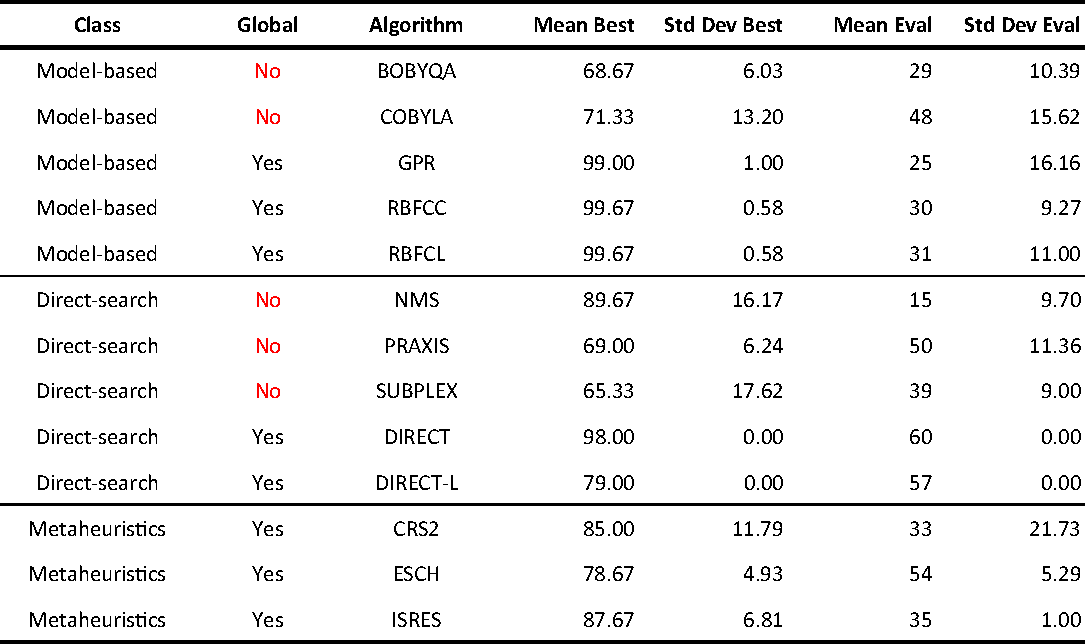
\includegraphics[width=\textwidth]{../report/tables_and_code/Ericeira_phase1_stats_v1.pdf}
\end{table}

\Cref{table:phase1results} shows the mean best results and the standard deviation of the three runs, discriminated by algorithm. According to the results, in average, the global model-based algorithms \textit{\ac{GPR}}, \textit{\ac{RBF}CC}, and \textit{\ac{RBF}CL} were able to find an optimal solution within the first $30$ evaluations. Conversely, the local model-based algorithms \textit{\ac{COBYLA}} and \textit{\ac{BOBYQA}} performed rather poorly in this problem, converging to far from optimal solutions after $29$ and $48$ function evaluations, respectively. Regarding direct-search algorithms, the global algorithm \textit{\ac{DIRECT}} was able to find a close to optimal solution (with an \ac{sUDI} value of $98\%$) in the last function evaluation. Its local variant, \textit{\ac{DIRECT}-L}, and the local direct-search algorithms \textit{\ac{PRAXIS}} and \textit{SUBPLEX} fell short of the expected and barely managed to improve over $80\%$. Nevertheless, the simplex-based direct-search algorithm \textit{\ac{NMS}} performed surprisingly well, having achieved an average result of $89.67\%$ within the first $15$ evaluations. Finally, although metaheuristics performed better than most local model-based and direct-search algorithms, they seem to stagnate in design solutions with \ac{sUDI} values below the $88\%$, after $30$ evaluations.

\Cref{fig:phase1results} shows the average performance per algorithm class, also separating them in local or global algorithms. Overall, local algorithms seem to perform worse than all other algorithms, with local direct-search and model-based algorithms stagnating towards design solutions with \ac{sUDI} values below $75\%$ and $70\%$, respectively. Contrastingly, global algorithms were able to find design solutions with values of \ac{sUDI} larger than $80\%$. Despite the good initial performance of metaheuristics algorithms for the first $20$ evaluations, global direct-search algorithms quickly surpassed them, achieving close to optimal solutions with \ac{sUDI} values of $90\%$. Lastly, global model-based algorithms were, on average, the best performing algorithms, achieving close to optimal solutions shortly after $24$ evaluations. 

\begin{figure}[htbp]
	\centering
	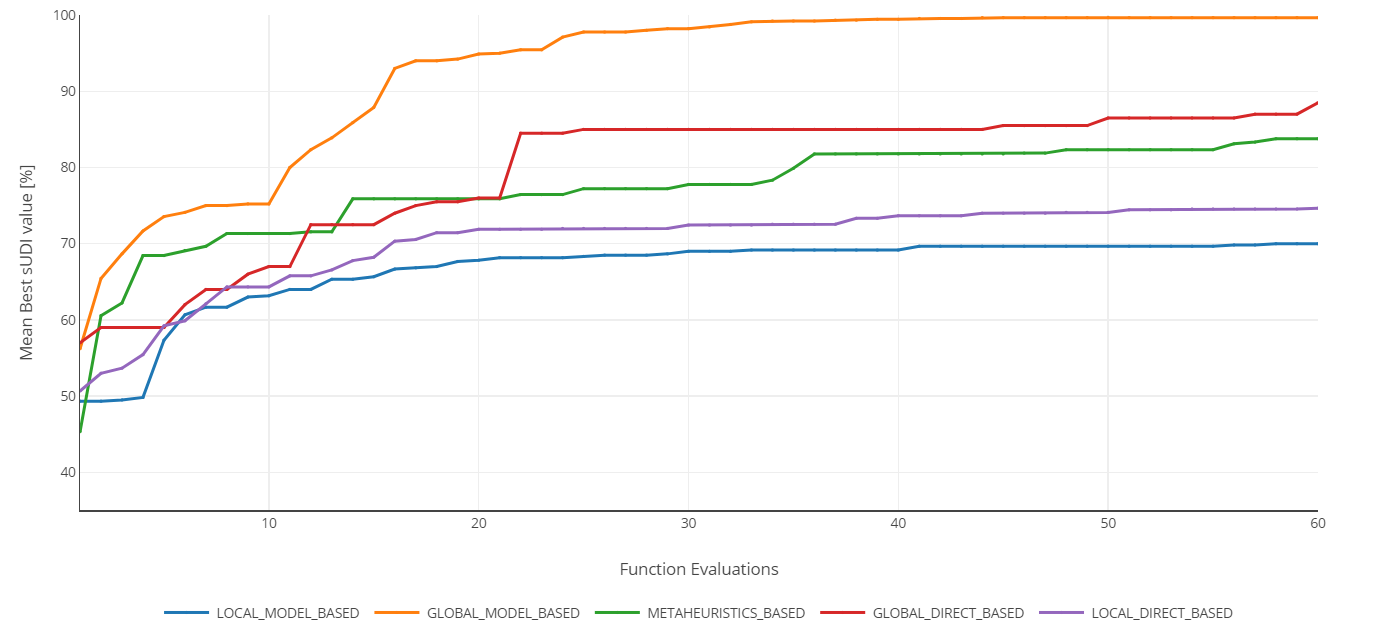
\includegraphics[width=1\textwidth]{../report/Images/Evaluation/Ericeira_results_ph1_per_class.PNG}
	\caption[Ericeira Solarium: Mean best daylight results in function of the number of evaluations, discriminated per class of algorithms]{Ericeira Solarium: Mean best daylight results in function of the number of evaluations, discriminated per class of algorithms.}
	\label{fig:phase1results}
\end{figure}

Given the overall bad performance of local algorithms, we decided to assess their performance when initialized with different solutions. Notwithstanding their ability to quickly converge to locally optimal solutions, the quality of the found solutions highly depends on the solution used to initialize the search. Therefore, we have also studied the impact of different initial solutions in the performance of these algorithms. To this end, we tested all $5$ local algorithms with two different initial solutions: a bad solution, with a $7\%$ value of \ac{sUDI}, and a reasonable solution with a $78\%$ value of \ac{sUDI}. Moreover, we decided to further restrict the number of evaluations to $15$, thus emulating an hypothetical scenario, where users lack knowledge about different optimization algorithms and opt for testing several of them. Ideally, this would allow them to infer the most promising algorithm and obtain a reasonable solution to hot-start other algorithms and, potentially, improve the overall optimization time.

\Cref{fig:phase2results} presents the mean best daylight results found by each local optimization algorithm. As expected, no local algorithm was able to obtain a good solution when provided with a bad starting solution. On the one hand, when provided with a mild initial design, both \textit{\ac{COBYLA}} and \textit{\ac{NMS}} found the best designs achieving a \ac{sUDI} value of $99\%$. On the contrary, \textit{\ac{PRAXIS}} found the worse, and showed no relevant improvement over the initial design. Nevertheless, it initially managed to outperform other methods, achieving values of \ac{sUDI} of $80\%$. After $8$ evaluations, \textit{\ac{COBYLA}} and \textit{\ac{NMS}} quickly converged to near optimal designs, with \ac{sUDI} values of $99\%$ and $98\%$, respectively. \textit{\ac{BOBYQA}} and \textit{SUBPLEX} struggled to improve from the initial design.
\begin{figure}[htbp]
	\centering
	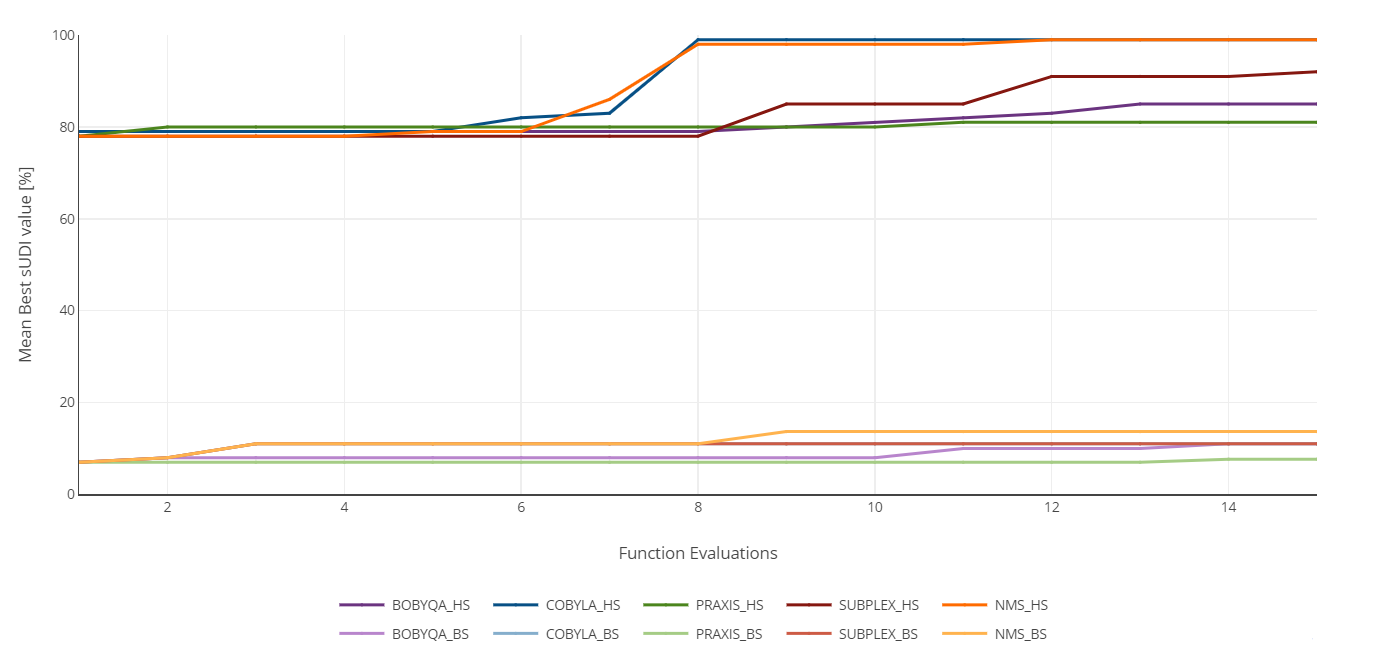
\includegraphics[width=\textwidth]{../report/Images/Evaluation/Ericeira_results_ph2.PNG}
	\caption[Ericeira Solarium: Mean best results of daylight performance in function of the number of evaluations, discriminated per local algorithm]{Ericeira Solarium: Mean best results daylight results as a function of the number of function evaluations, discriminated per local algorithm. Algorithms suffixed with \textit{HS} are given an initial solution with an \ac{sUDI} value of $78\%$, whilst algorithms suffixed with \textit{BS} are given an initial solution with an \ac{sUDI} value of $7\%$.}
	\label{fig:phase2results}
\end{figure}

On the other hand, when provided with a bad initial design, the best daylight result has an \ac{sUDI} value of $15\%$ and was found by \textit{\ac{NMS}} after $9$ evaluations. \textit{\ac{NMS}}, \textit{\ac{COBYLA}}, and \textit{SUBPLEX} exhibit similar performance, stagnating in a design with an \ac{sUDI} value of $11\%$ after $3$ evaluations, with \textit{\ac{NMS}} being able to further improve the design after $5$ evaluations. \textit{\ac{PRAXIS}} exhibits the worst performance among all methods, showing no significant improvements throughout the whole optimization process.


\subsection{Multi-Objective Optimization: Space Frame Optimization}
In this section, we evaluate two \ac{MOO} problems \cite{Belem2019MOO,IP2019MOO}. As previously discussed in \cref{ssec:performance}, addressing these problems comprises a difficult task, not only because of the higher complexity of the obtained results, but also because of the absence of standards regarding the best way to evaluate the \acp{MOOA}' performance. For these reasons, in this dissertation, we opted for evaluating the algorithms' performance in terms of the results returned by each algorithm, i.e., the \acp{aPF}. For each algorithm, we compute different indicators that measure the \acp{aPF} in terms of their cardinality, diversity, and accuracy.%: \ac{ONVGR}, \ac{ER}, Spacing, Maximum Spread, \ac{MPFE}, \ac{GD}, and \ac{HV}. 

Although some indicators measure aspects based exclusively on the \acp{aPF}, others require a reference set to compare with the \acp{aPF}. Ideally, this reference set would represent the real optimal solutions for the specified problem. Unfortunately, this set of optimal solutions, also called \ac{tPF}, is not known for most \ac{BPO} problems. In an attempt to better approximate it, we compute a fictitious Pareto Front, the \ac{cPF}, composed of the best solutions found by each algorithm. 

Note, however, that we aimed at measuring the average performance of each algorithm regarding an unknown \ac{tPF}. In general, computing an accurate approximation of the \ac{tPF} would require running the algorithms for thousands of iterations, which is not feasible in most \ac{BPO} problems involving time-consuming evaluation functions. As a consequence, we adopted a methodology similar to the one used in \cref{ssec:soocasestudy}, which quantifies the performance of each algorithm in terms of the mean value of three runs, using as reference, for each run, the corresponding \acp{cPF}. 

In the next sections, we present and discuss the obtained results for each algorithm. In \cref{appendix:appendixB}, we provide additional information about each algorithm's configuration and present the Pareto front plots corresponding to each run.

\subsubsection{Space Frame Optimization}
Motivated by the interest of architects in performing structural analysis \cite{Cichocka2017SURVEY}, the first \ac{MOO} case study consisted in the optimization of both the structural behavior and an \textit{ad-hoc} measure of the irregularity of an arc-shaped space frame. To instil irregularities in the space frame, we introduced three attractors that cause a deformation in the shape of the truss, each of which is defined in terms of its fixed-radius cylindrical coordinates in the arc-shaped space frame~\cite{Belem2019MOO}. To measure the goals for each design variant, we used (1) the Robot analysis tool to compute the maximum displacement of the structure, and (2) the sum of the Euclidean distances between the attractors. To increase the interest of this case study, we set out to minimize both objectives, thus promoting the conflict between them: placing the attractors near each other will weaken the structure and, thus, increase the maximum displacement of the space frame. In fact, to reduce the maximum displacement, the attractors should be scattered across the space frame but this implies larger distances among the three attractors, thus worsening the second objective. \Cref{fig:spaceframe} illustrates three examples of the space frame structure. 
\begin{figure}[htbp]
	\centering
	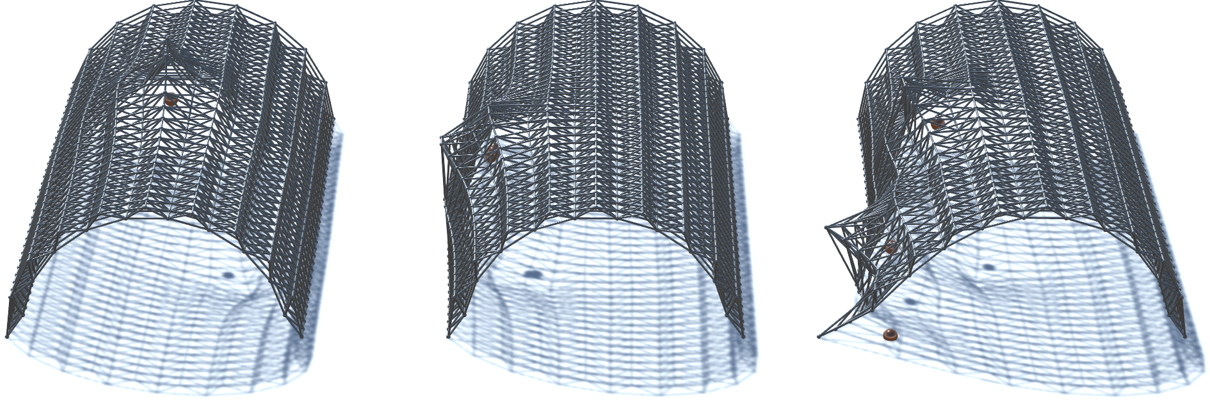
\includegraphics[width=1\textwidth]{../report/Images/Evaluation/truss-kat-small.png}
	\caption[Space Frame: Representation of three space frame design variants]{Space Frame: Representation of three design variations of the arc-shaped space frame, with copper balls representing the three attractors.}
	\label{fig:spaceframe}
\end{figure}

To optimize the space frame, we decided to test $10$ metaheuristics and $9$ model-based algorithms. On the one hand, each metaheuristic algorithm comprised a total of $15$ individuals/particles per iteration, which were evolved for $15$ iterations. On the other hand, model-based algorithms derived $100$ initial samples using the Latin Hypercube sampling algorithm, which were then used to create the initial approximation to the expensive evaluation function, upon which another $125$ evaluations were completed. Overall, every algorithm was limited to a total of $225$ function evaluations, each taking approximately $40$ seconds to complete on a dual \textit{Intel Xeon CPU E5-2670 @ 2.60GHz with 64GB RAM}. In total, each run is composed of $4275$ candidate solutions and takes approximately $2$ days to complete.

\Cref{table:spaceframe,table:spaceframestd} show the mean results of the performance indicators and corresponding standard deviations for the three runs, discriminated by the algorithms' classes and subclasses. As previously mentioned, we computed several performance indicators for each \ac{aPF}, which provide information about: (1) cardinality, measured by \ac{ONVGR} and \ac{ER}; (2) diversity, measured with Spacing and Maximum Spread; and (3) accuracy/convergence, measured with \ac{MPFE} and \ac{GD}. Moreover, we used a Pareto-compliant indicator, the \ac{HV}, to obtain a combined measure of all the three mentioned aspects. % To simplify the performance comparison among the different algorithms, we restrained the set of indicators to the unary ones. 
% 1 - Two set coverage não ia dar medidas relevantes porque raramente as diferentes frentes se tocam. 
% 2 - Epsilon indicators poderia ser interessante, mas não foi testada a implementação
% 3 - R-metrics requer funções de utilidade que não temos e que requer alguma sensibilidade em relação ao problema...

% The overall cardinality of each combined Pareto front is 14, 24, and 19, respectively.
When considering the cardinality aspect, the \ac{ONVGR} column of \cref{table:spaceframe} presents the ratio of optimal solutions between \acp{aPF} and \acp{cPF}. In general, metaheuristics seem to retrieve the most nondominated solutions within each run, whereas model-based algorithms seem to retrieve the least. In fact, among the model-based algorithms, the algorithms exploring random search strategies, i.e., the algorithms suffixed with \textit{Random}, yield fewer nondominated solutions, which may result from a poor exploration of the solution space. On average, the best performing algorithm, \textit{PAES}, is able to find twice the number of solutions that compose each \ac{cPF}, whereas model-based algorithms, including \textit{GPR+Random} and \acp{MLP} algorithms, struggled to find a set of optimal solutions with at least half of the size of the \acp{cPF}. 
%http://papers.cumincad.org/data/works/att/caadria2018\_278.pdf
\begin{table}[h!]
	\centering
	\caption[Space Frame: Mean values for the performance indicators results, discriminated per algorithms]{Space Frame: Mean values for the performance indicators results, discriminated by algorithm. Results are averaged over $3$ runs, each with $225$ evaluations.}
	\label{table:spaceframe}
	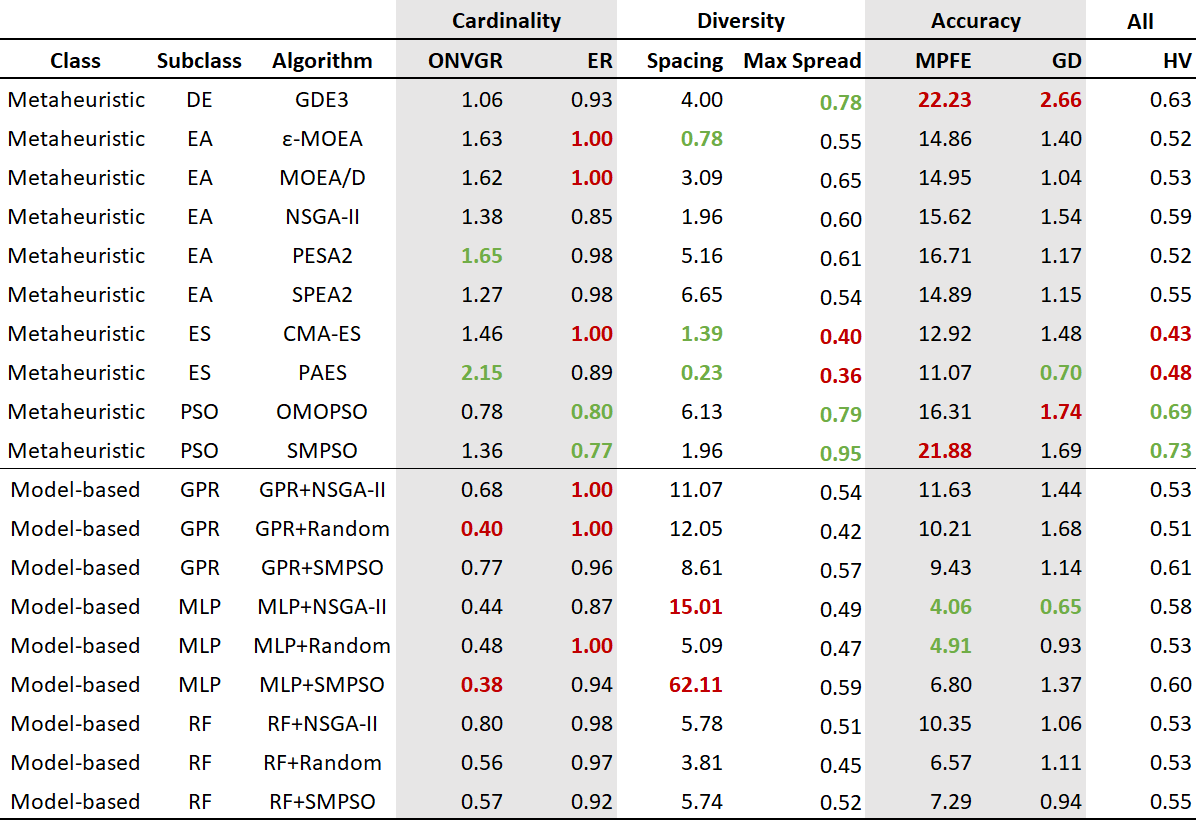
\includegraphics[width=\textwidth]{../report/Images/Evaluation/caadria/Results_Mean_20190428.PNG}
\end{table}

While the \ac{ONVGR} indicator provides an intuition about the richness of each algorithm's \acp{aPF}, many of the identified solutions might not be truly optimal, i.e., despite being optimal among all the evaluated solutions, these solutions might not belong to the corresponding \ac{cPF}. To this end, \ac{ER} is used to measure the percentage of false-optimal solutions for each algorithm. In this case, it becomes clear that even though \textit{PAES} retrieves twice as many optimal solutions as the \acp{cPF}, most of them are not truly optimal. Moreover, none of the solutions found by the $\epsilon$\textit{-MOEA}, \textit{MOEA/D}, and \textit{CMA-ES} metaheuristics algorithms belong to the \acp{cPF}. The same happens with some of the model-based algorithms, particularly, \textit{GPR+NSGA-II}, \textit{GPR+Random}, and \textit{MLP+Random}. On the other hand, \ac{PSO}-based metaheuristics algorithms, \textit{SMPSO} and \textit{OMOPSO}, exhibit the lowest \ac{ER} value, having found at least one optimal solution in each run.

The diversity aspect consists in the analysis of the distribution of the nondominated solutions across the objective space. The Spacing indicator measures the uniformity of the \acp{aPF}, regardless of the \acp{cPF}. Considering this indicator, the two \ac{ES} metaheuristic algorithms, \textit{PAES} and \textit{CMA-ES}, and one \ac{EA}-based metaheuristic algorithm, $\epsilon$\textit{-MOEA}, achieved the most uniform \acp{aPF}. Conversely, model-based algorithms seem to yield more irregular \acp{aPF}, namely, \textit{MLP+NSGA-II} and \textit{MLP+SMPSO} achieved the worst values of the Spacing indicator. Note, however, that this indicator merely provides an idea of the regularity of distribution of the solutions. Ideally, this indicator would also suggest a good coverage of the \ac{cPF}, i.e., that the \acp{aPF} found by each algorithm cover the same regions as the \acp{cPF}, instead of focusing on narrower regions. However, most of the algorithms that present the best Spacing scores achieve such values because most of the identified optimal solutions lie within the same small region but present a more uniform distribution. Besides this limitation, these indicators are also highly sensitive to outliers and to the number of retrieved solutions. % number of solutions also indirectly contributes to these scores of each indicators, since these indicators measure the distances between consecutive optimal solutions and the weight each outlier has in smaller or larger sets can greatly influence the final result.

Besides having an uniform distribution, when applicable, good Pareto fronts should also cover large extents of the objective space in order to provide more relevant trade-offs. \textit{Max Spread} measures the extent of the \acp{aPF} retrieved by each algorithm. On average, \textit{SMPSO}, \textit{GDE3}, and \textit{OMOPSO} are able to explore wider extents of the objective space. Observing \cref{table:spaceframe}, we conclude that, on average, \textit{SMPSO}, \textit{GDE3}, and \textit{OMOPSO} were able to cover the objective space better. Contrastingly, the \ac{ES}-based algorithms were the worst algorithms in this aspect, having explored smaller regions of the objective space. Regarding model-based algorithms, it is possible to observe that the ones based on \textit{SMPSO} were able to explore broader regions of the objective space than the ones based on \textit{NSGA-II} or \textit{Random} strategies. 
\begin{table}[]
	\centering
	\caption[Space Frame: Standard deviation values for the performance indicators results, discriminated by each algorithm]{Space Frame: Standard deviation values for the performance indicators results, discriminated by algorithm. Results are averaged over $3$ runs, each with $225$ evaluations.}
	\label{table:spaceframestd}
	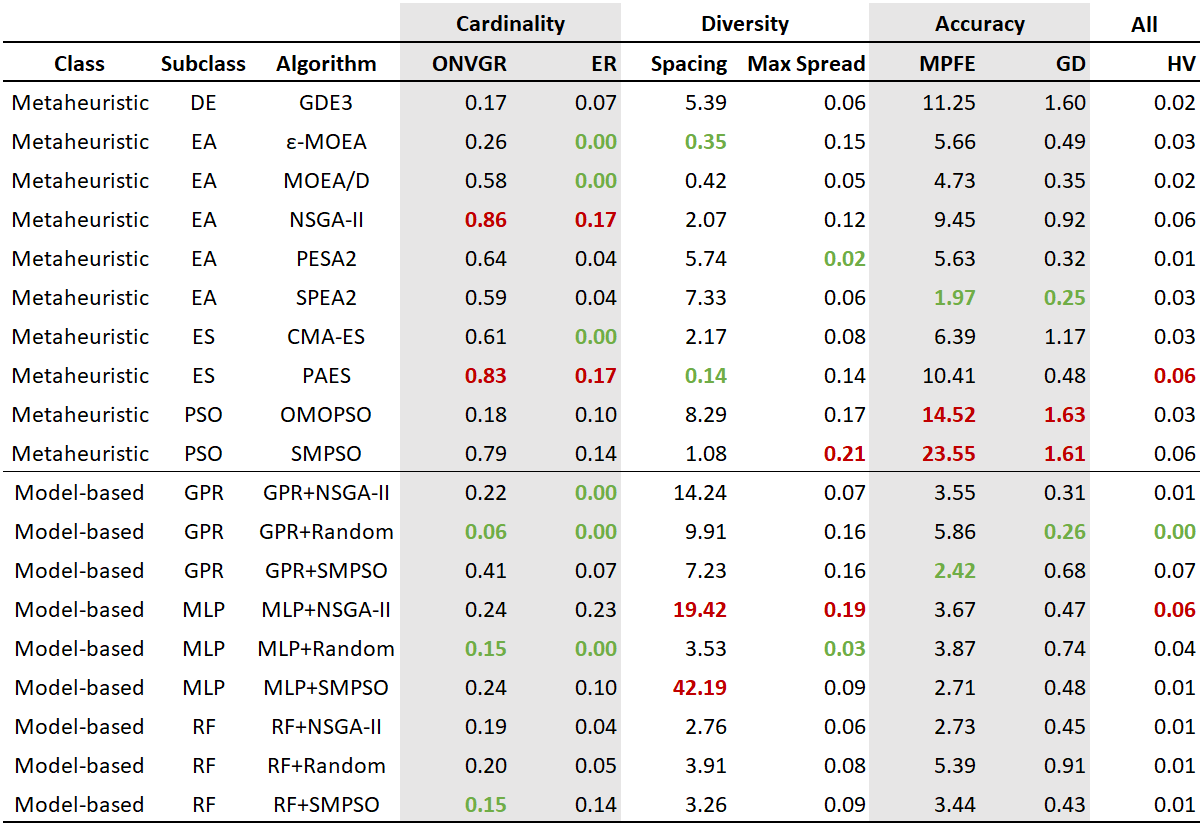
\includegraphics[width=\textwidth]{../report/Images/Evaluation/caadria/Results_Std_20190428.PNG}
\end{table}

Another important aspect of \acp{aPF} is their accuracy and how close their solutions are from the \acp{cPF}. In this case study, we considered two accuracy indicators, \ac{MPFE} and \ac{GD}. On average, when considering \ac{MPFE}, every model-based algorithm retrieved \acp{aPF} whose \ac{MPFE} values were always better than the ones obtained by any metaheuristic. In particular, \textit{MLP+NSGA-II} and \textit{MLP+Random} have the smallest maximum error which means that all the points are at most at that distance from an optimal solution. Furthermore, the algorithms exploring a larger extent of the objective space, i.e., with higher values of Max Spread, have worse \ac{MPFE} values. This can be explained due to the lack of information about the \ac{tPF}, which is only being approximated by the best solutions found in each run, i.e., the \acp{cPF}. 

Notwithstanding the fact that \ac{MPFE} provides an estimate of the maximum error of the algorithms' \acp{aPF}, this indicator does not provide a real measure of how close the results are to the \acp{cPF}. To this end, we use the \ac{GD} indicator, which measures the average approximation of the \acp{aPF} retrieved by each algorithm to the closest solutions in the corresponding \acp{cPF}. \Cref{table:spaceframe} shows that, on average, \textit{MLP+NSGA-II} and \textit{PAES} present the best convergence towards the \ac{cPF}, and that \textit{GDE3} and \textit{OMOPSO} present the worst convergence values. These can be explained by the number of the nondominated solutions retrieved by each algorithm, as well as by the creation of clusters of optimal solutions near the \acp{cPF} that were discovered by \textit{PAES} and \textit{MOEA/D}, as is visible in \cref{sec:spaceframeoptimizationextra}. In general, other model-based algorithms also present reasonable scores, like the \textit{MLP+Random} or all the \ac{RF}-based algorithms even surpassing many metaheuristics algorithms, including \textit{CMA-ES}, $\epsilon$\textit{-MOEA}, \textit{NSGA-II}, and \textit{SPEA2}, thus suggesting better approximations.

In the end, we also used the \ac{HV} indicator, as it appraises the quality of a Pareto front with regards to all three aspects simultaneously. The best performing algorithms were the \ac{PSO}-based algorithms, \textit{SMPSO} and \textit{OMOPSO}, followed by \textit{GDE3}. Surprisingly, the \ac{PSO} model-based algorithms also present a good performance, when compared to other metaheuristics, and even to other model-based algorithms that explore \textit{Random} or \ac{EA} strategies to search for optimal solutions. Conversely, the worst performing algorithms were the \ac{ES}-based ones, \textit{CMA-ES} and \textit{PAES}, followed by \textit{GPR+Random}. % Finally, comparing different algorithms regarding \ac{IGD}, the \ac{PSO}-based metaheuristic algorithms still yielded the best results, whilst \ac{ES}-based metaheuristic algorithms yielded the worst. However, \textit{MOEA/D} unexpectedly reveals itself as the third best performing algorithm when considering the \ac{IGD} indicator. Although this seems odd, this value can be explained by the difference in the scales of both axis and to the higher density of Pareto optimal solutions in the $x$-axis for values between $1.2$ and $1.3$.
\begin{figure}[hptb]
	\centering
	\includegraphics[width=\textwidth]{../report/Images/Evaluation/caadria/All_Algorithms_all_runs-2019-04-13_1000dpi.png}
	\caption[Space Frame: Pareto front plot]{Space Frame: Algorithms' \acp{aPF} measuring the attractors distance, in function of the maximum displacement. These fronts are obtained by combining the values of the $3$ runs for each algorithm. The \ac{cPF} is formed by finding the nondominated solutions from all the evaluated solutions.}
	\label{fig:allruns}
\end{figure}

Overall, no single algorithm was able to outperform the others in terms of all the indicators. Nevertheless, the \ac{PSO}-based metaheuristics algorithms, \textit{OMOPSO} and \textit{SMPSO}, exhibited the overall best performance. Moreover, even though none of the model-based algorithms was able to surpass the \textit{SMPSO} and \textit{OMOPSO}, the model-based algorithms that use \textit{SMPSO} also exhibited a reasonable performance, better than several well-known metaheuristics, including $\epsilon$\textit{-MOEA}, \textit{MOEA/D}, \textit{CMA-ES}, and \textit{SPEA2}. \Cref{fig:allruns} presents a combined view of all the algorithms for every run, where it is possible to visualize the extent of \ac{PSO}-based algorithms and the high density region to which several \acp{EA} and \acp{ES} algorithms converged.

	\section{Conclusions}
\label{sec:concl}

Nowadays, with the threat of climate change, resource depletion, and worldwide urbanization, it is not enough to construct well-designed buildings, it is also necessary to optimize them \cite{Wortmann2015AdvSBO}. Architectural practices have, therefore, grown to incorporate considerations about the building's performance in various aspects. The development of computational simulation tools empowered designers with the ability to simulate and estimate a building’s performance. The emergence of these tools and the raising concerns about the environmental and economic impact of buildings led to the development of new design approaches, such as \ac{PBD}, which seek more efficient design solutions by considering the designs’ performance. Taking \ac{PBD} a step further, optimization has unveiled a new performance-based approach called \ac{BPO}. 

Unfortunately, traditional \ac{BPO} methodologies require the evaluation of different design variations, which, in turn, implies spending a large amount of time with the manual application of changes to the design and often leading to difficulties when modeling complex geometry. Moreover, in order to evaluate a design's performance, the corresponding analytical models must be produced, which also comprises a time-consuming and tiresome task. The emergence of algorithmic-based paradigms, like \ac{AD} and \ac{AA}, enabled the implementation of automated optimization processes, as they allow architects to generate multiple design variants with little effort, to automatically produce the corresponding analytical models, and to automatically evaluate their performance. 

Optimization algorithms can be coupled with the previously mentioned algorithmic approaches and simulation tools to more efficiently seek for optimal design solutions. Given that a single evaluation may take a considerable amount of time to complete, in order to speed up the optimization process, it becomes necessary to identify the optimization algorithms capable of handling the computationally complex problems that characterize \ac{BPO}, and to devise strategies for its efficient application in architecture. Often disregarded, the selection of the appropriate optimization algorithm can have a significant impact in the overall efficiency of optimization processes, and also on the quality of the results \cite{Wolpert1997NFLT}.

However, most \ac{BPO} practitioners adopt the simplest available algorithm, such as \acp{EA} \cite{Evins2013}, which typically require several hundreds or thousands of evaluations - an infeasible scenario for most \ac{BPO} problems. Conversely, direct-search and model-based algorithms are more promising, frequently yielding better results in fewer evaluations \cite{Waibel2018}. Particularly, model-based algorithms can considerably reduce the time spent in optimization \cite{Wortmann2017GABESTCHOICE}. Moreover, obtained results exhibit an average reduction by about $50\%$ on the total time spent in optimization, when using model-based algorithms.

Along these lines, we addressed optimization algorithms specifically tailored for handling simulation-based optimization problems, where the computational effort associated to each simulation often restricts number of function evaluations to a few dozens or hundreds. We introduced \ac{AO}, an extension to the \ac{AD} and \ac{AA} approaches, that combines an optimization framework with an \ac{AD} tool to facilitate users to address various design optimization problems, including \ac{BPO}. Results show that no single class, subclass, or algorithm excels at every problem, thus corroborating the \acp{NFLT} for optimization \cite{Wolpert1997NFLT}. 

Moreover, even though most tools rely on \ac{GA}-based algorithms, these rarely achieved the best performance in the evaluated case studies. Instead, other categories, such as model-based or direct-search algorithms, yielded better results. Different factors could change the obtained results (e.g., a different configuration for the algorithms or a lucky random step). Therefore, and contrarily to current architectural practices, we conclude that distinct algorithms behave differently according to the problems' characteristics and that architects should test various algorithms for a small number of evaluations or for a short amount of time. 
Furthermore, we also conclude that while global optimization algorithms are quicker to converge towards optimal solutions when no additional information is known, local algorithms can be quicker if provided with good starting points and, therefore, should be considered as potential candidates when such information is available.

Regarding the evaluation of different \acp{MOO} algorithms, the lack of consensus regarding the more appropriate way to measure their quality makes it difficult to quantify the suitability of each algorithm for \ac{MOO} problems. We conclude that algorithms' quality should be measured through the combination of Pareto front plots and multiple \ac{MOO} performance indicators. Particularly, some indicators should provide a measure of the diversity of the nondominated solutions across the solution space, while others should measure the overall accuracy of the results.

To bypass the identified limitations, the proposed optimization framework includes different categories of optimization algorithms and facilitates their application by abstracting them under a common interface, thus promoting automated optimization processes. To further facilitate the selection of the most appropriate algorithm, it also includes mechanisms to test multiple algorithms effortlessly. The suitability and capabilities of the framework were evaluated in the context of two \ac{BPO} problems, which demonstrated its ability to solve real architectural problems characterized by computationally complex objective functions.

Overall, optimization can be very beneficial for architecture. The combination of simulation tools, algorithmic-based approaches, and optimization algorithms enables the automation of optimization processes within architectural practices. Despite its benefits, the incorrect application of these optimization processes can lead to poor results. Moreover, distinct architectural design problems benefit most from different optimization algorithms, capable of handling them more efficiently. However, most architectural optimization tools focus on the same subset of algorithms, which are rarely the most adequate algorithms. The proposed framework circumvents these limitations by presenting several optimization algorithms with different characteristics, thus fostering better optimization practices. Finally, the proposed \ac{AO} methodology was shown to benefit the architectural practice, as demonstrated by the case studies.

% REFERENCES

% Produces the bibliography section when processed by BibTeX
%
% Bibliography style
% > entries ordered alphabetically
%\bibliographystyle{plain}
% > unsorted with entries appearing in the order in which the citations appear.
%\bibliographystyle{unsrt}
% > entries ordered alphabetically, with first names and names of journals and months abbreviated
\bibliographystyle{abbrv}
% > entries ordered alphabetically, with reference markers based on authors' initials and publication year
%\bibliographystyle{alpha}

% External bibliography database file in the BibTeX format (ExtendedAbstract_ref_db.bib)
\bibliography{references}

\end{document}


